\documentclass[a4paper,10pt]{article}
\usepackage[utf8x]{inputenc}
\usepackage[ngerman]{babel}
\usepackage{cite}

\newcommand{\rem}[1]{}


%opening
\title{Die Pioneer-Anormalie}
%\author{Judith Selig\footnote{judith.selig@gmx.de}, Michael F. Schönitzer\footnote{michael@schoenitzer.de}, Florian Schlagintweit\footnote{florian@schlagintweit.de}}	% welche Reihenfolge der Namen?
%\author{Judith Selig\thanks{judith.selig@gmx.de}, Michael F. Schönitzer\thanks{michael@schoenitzer.de}, Florian Schlagintweit\footnote{florian@schlagintweit.de}}	% welche Reihenfolge der Namen?

\author{Judith Selig\\judith.selig@gmx.de \and Michael F. Schönitzer\\michael@schoenitzer.de \and Florian Schlagintweit\\florian@schlagintweit.de}	% welche Reihenfolge der Namen?


\begin{document}

\maketitle

% \begin{abstract}

% \end{abstract}



\section{Geschichte}

Im Februar 1969 genehmigte die NASA ( National Aeronautics and Space
Administration) ein Programm, um den Asteroideng\"urtel, das
interplanetare Medium zwischen Mars und Jupiter, die \"au{\ss}eren
Planeten und Fly-By Man\"over zu erforschen. Hierzu wurden zwei
baugleiche Sonden Pioneer F (Pioneer 10 Mission) und Pioneer G (Pioneer
11 Mission) zum Jupiter gebracht. Die Pioneer 10 Mission startete am 2.
M\"arz 1972 und wurde dann auf ca. 14,4 km/s beschleunigt. Die Sonde
durchflog im Juli 1972 unbeschadet den Asteroideng\"urtel und erreichte
am 4. Dezember 1973 den Jupiter. Hier nutzte man ein Fly-By Man\"over
um die Sonde auf eine heliozentrische Fluchtgeschwindigkeit von 11,322
km/s (Gesamtgeschwindigkeit 36,7 km/s)zu beschleunigen um das
Sonnensystem in Richtung des Sterns Aldebaran (Laut Zeitplan sollte die
Sonde den Stern in ungef\"ahr 2 Millionen Jahren erreichen\cite{Nieto2007}) zu verlassen. Pioneer
11 startete 13 Monate sp\"ater, am 6. April 1973, da die NASA mit
Pioneer 10 erst herausfinden wollte, ob eine Durchquerung des
Asteroideng\"urtels \"uberhaupt m\"oglich ist. Ihre Bahn f\"uhrte
Pioneer 11 ebenfals Richtung Jupiter, den sie am 2. Dezember 1974
erreichte. Das dort durchgef\"uhrte Fly-By Man\"over brachte sie auf
eine Bahn, die Pioneer 11 zun\"achst wieder innerhalb der Jupiter-Bahn
f\"uhrte, um dann aber am 1. September 1979 den Saturn zu erreichen
(Abb. \$1) In einem weiteren Fly-By Man\"over, bei dem die Sonde die
Ringe des Saturns unbeschadet durchquert hat, wurde sie auf eine
asymptotische Fluchtgeschwindigkeit von 10,450 km/s gebracht. Pioneer
11 steuert auf die Konstellation Aquila zu, wo sie in ungef\"ahr 4
Millionen Jahren eintreffen wird. Die Relationen der Flugbahnen der
Sonden Pioneer 10 und 11, sowie Voyager 1 und 2 sind in Abb. \$2 zu
erkennen.


\bigskip

Abb. \$1 und \$2


\bigskip

Obwohl Pioneer 10 und 11 nur auf eine Betriebszeit von 21 Monate
ausgelegt waren, sendete Pioneer 10 Messdaten bis zum 27. April 2002.
Das letzte Signal von Pioneer 10 erreichte die Erde am 23. Januar 2003.
Das letzte Signal von Pioneer 11 wurde jedoch deutlich fr\"uher, am 24.
November 1995 empfangen, da durch das zweite Fly-By Man\"over am Saturn
sehr viel mehr Leistung ben\"otigt wurde.

Zu den o.g. Missionszielen geh\"orte vor allem unter dem Ziel der
Erforschung der \"au{\ss}eren Planeten die Suche nach dem
{\quotedblbase}Planeten X``, der damals jenseits von Neptun vermutet
wurde. Um das schwache Gravitationsfeld dieses omin\"osen Planeten
nachzuweisen und um m\"oglichst nahe an Jupiter und Saturn vorbei zu
fliegen, ben\"otigten die Pioneer-Sonden eine sehr genaue Navigation.
Dabei wurden von einer Bodenstation des Deep Space Network DSN (in
Goldstone/USA, Madrid/Spanien, Canberra/Australien) Radiowellen mit
einer wohldefinierten Frequenz zur Sonde geschickt. Die Pioneers
sendete dieses Signal mit einer um den Faktor 240/221 konvertierten
Frequenz wieder zur Erde zur\"uck\cite{Dittus2006}.
Diese genaue Navigation erlaubte schlie{\ss}lich die Entdeckung der
Pioneer-Anomalie. 

Damit die Parabolantenne immer auf die Erde gerichtet blieb, musste
die Sonde vor allem nach Vorbeifl\"ugen an gro{\ss}en Planeten neu
ausgerichtet werden. Hierzu wurden kleine Triebwerke f\"ur eine kurze
Zeit gez\"undet. Alle weiteren St\"orfaktoren auf die Flugbahn von
Pioneer 10 und 11 wurden mit einer Eigenrotation der Sonden um die
Symmetrieachse der Parabolantenne von 4 bis 7 U/min
ausgeglichen\cite{Dittus2006} \cite{Nieto2007}.

Durch die genaue Navigation und die Verminderung von Fehlern,
bemerkte man Anfang der 80-er eine unvorhergesehene Beschleunigung von 
$(8,74\pm 1,33)\cdot 10^{-8}\mathit{cm}/s^{2}$ \cite{Anderson2002} in Richtung der Sonne. 

Diese Beschleunigung wurde schlie{\ss}lich zur Pioneer-Anomalie, deren
Ursache bis heute nicht bekannt ist. 

\section{Die Anomalie}

\subsection{Navigation und Geschwindigkeitsmessung}
Die Navigation der Pioneersonden erfolgte mithilfe der Antennen des Deep Space Network (DSN) einem Zusammenschluss mehrerer Radioteleskopanlagen des Jet Propulsion Laboratory (JPL)\footnote{Das Jet Propulsion Laboratory in Kalifornien entwickelt und steuert Sonden für die NASA und beschäftigt viele der Experten auf dem Gebiet der Pioneeranomalie, darunter auch John D. Anderson und Slava G. Turyshev}. Das DSN besteht heute aus großen Radioteleskopanlagen in Goldstone/USA, Madrid/Spanien und Canberra/Australien. Früher gab es darüber hinaus noch Anlagen in Woomera/Australien und Johannesburg/Süd Afrika.\cite{Anderson2002}\cite{Turyshev2010} Dies sind jeweils Komplexe von zahlreichen Antennen – für die Navigation der Pioneer-Sonden wurden laut der Arbeit von Anderson et al., 2002\cite{Anderson2002} davon die Deep Space Station (DSS) Antennen 12, 14, 42, 43, 62 und 63 verwendet. Turyshev und Toth erläutern jedoch in ihrer 2010 erschienenen Arbeit, dass noch etliche weitere Antennen auf alle Parks des DSN, sowie auch einige Antennen anderer Einrichtungen verwendet wurden.\cite{Turyshev2010} Die Antennen hatten Anfangs meist Durchmesser von 26 Metern, später häufig 34 oder 64 Meter teilweise bis zu 70 Meter.\cite{Turyshev2010}
Man sollte erwähnen, dass diese Antennenkomplexe im laufe der Zeit zahlreich umgebaut wurden um den Anforderungen neuer Missionen gerecht zu werden. Dabei haben sich unter anderem auch die internen Frequenzen geändert\cite{Anderson2002}. Dies muss bei der genauen Betrachtung der Daten berücksichtigt werden, ist darüber hinaus jedoch auch eine Voraussetzung für die 30 Jahre lange Missionsdauer gewesen, da ansonsten die Reichweite der Antennen nur bei etwa 22 AU gelegen hätte.\cite{Turyshev2010}
Die Geschwindigkeitsmessung der Pioneersonden, welche für die Pioneeranomalie von zentraler Bedeutung ist, erfolgte über die Zwei-Wege-Dopplerverschiebung von Radiowellen:

Wir nehmen im folgenden an, dass die Sonde sich näherungsweise radial von uns wegbewegt.
Von den Bodenstationen wurden Radiowellen bekannter Frequenz (S-Band, $\sim$2,11 GHz) zum Satelliten gesendet (uplink).
Die Frequenz wird mithilfe eines Wasserstoff-Masers erzeugt.
Damit wird eine äußerst präzise und stabile Referenz-Frequenz von 5 MHz und 10 MHz erzeugt. Im Digital Controlled Oscillator (DCO), werden diese Frequenz verwendet um mit frequenzmultipliern ein Signal mit ungefähr 22 MHz zu erzeugten, welches dann mit dem Faktor 96 multipliziert wird um das zu sendende Signal von etwa 2,11 GHz zu erhalten.\cite{Anderson2002}
Der Satellit empfängt das Signal dopplerverschoben:
\begin{equation}
 \nu_R = \frac{1}{\sqrt{1-\frac{v^2}{c^2}}}(1-\frac{v}{c})\nu_E
\end{equation}
und antwortet unmittelbar mittels einer 8-Watt Sendeanlage und eines Transponders
mit einer um den festen Faktor $ \frac{240}{221} $ multiplizierten Frequenz:
\begin{equation}
\nu'_R = \nu_R\frac{240}{221}
\end{equation}
Dies ist notwendig, da es sich bei den Radiosignalen um kohärente Wellen handelt und man so Verfälschungen durch Interferenz der Hin- und Rücklaufenden Wellen vermeidet.\cite{Anderson2002}
Beim Rückweg wird das Signal ein zweites mal identisch dopplerverschoben.
Das empfangene Signal ist also zweifach dopplerverschoben und um den Faktor $\frac{240}{221}$ verschoben.
\begin{equation}
 \nu'_E = \frac{1}{\sqrt{1-\frac{v^2}{c^2}}}(1-\frac{v}{c}) \cdot \frac{240}{211}\nu_R \, = \,
\frac{1}{1-\frac{v^2}{c^2}}(1-\frac{v}{c})^2 \cdot \frac{240}{211} \nu_E
\end{equation}
Die relative Verschiebung ergibt sich also zu
\begin{equation}
 \frac{\nu'_E-\nu_E}{\nu_E} = \frac{\frac{19}{221}- \frac{461}{221}\frac{v}{c}}{1+\frac{v}{c}}.
\end{equation}
In vielen Quellen wird die konstante Frequenzverschiebung durch die Elektronik der Quelle vernachlässigt, was zur
einfacheren Form von
\begin{equation}
 \frac{\nu'_E-\nu_E}{\nu_E} \approx -2\frac{v/c}{1+v/c} \approx -2 \frac{v}{c}
\end{equation}
führt.
Sind Sender- und Empfängerantenne die selben, so spricht man von einer zwei-Wege-Messung, wenn Sende und Empfängerantennen unterschiedlich sind spricht man von einer drei-Wege-Messung.\cite{Levy2009} Bei den drei-Wege Doppler-Messungen besteht die Gefahr, dass ein unbekannter Zeitunterschied zwischen den Antennen die Messung verfälscht, daher verwendete man diese Daten meist nicht.\cite{Anderson2002} %schon oben, als footnote?
Darüber hinaus lässt sich die Entfernung $d$ der Sonde auch durch die Laufzeit $\Delta t$ des Signales bestimmen:
\begin{equation}
 2d = c \Delta t
\end{equation}
Dafür wird der Uplink per Phasenmodulation mit einem Signal versehen und das von der Sonde zurückgesendete Echo beobachtet. (Der Transponder der Sonde demoduliert und filtert es um es beim Down-link wieder hinein zu modulieren.)
Dabei muss man beachtet, das durch das ständige senden solcher Modulierten Signale und die langen Laufzeiten es zu Verwelchslungsgefahr zwischen unterschiedlichen Signalen kommen kann. Dies muss von den Analyseprogrammen erkannt werden.

Somit hat man zwei voneinander unabhängige Messmethoden, was Konsitenzchecks,
Fehlerminimierung und Ausschluss einiger phänomenologischer Fehler ermöglicht. Nicht zuletzt kann man damit durch Frequenzfehler kommende falsche Dopplerdaten erkennen.\cite{Anderson2002}
Allerdings wurde dies laut \cite{Anderson2002} nur bei der Analyse der Daten von Galileo und Ulysses (siehe unten), nicht bei den Pioneersonden verwendet.

Aufgrund der Eigenrotation der Erde lässt sich außerdem aus der dadurch entstehenden Modulation der Doppler-Daten auch die 3 dimensionale Position der Sonde berechnen. Die Amplitude der Sinusförmigen Variation ist mit dem Deklinationswinkel und die Phase mit der Rektaszension verbunden. Die Position lässt sich dadurch aus einem Satz Dopplerdaten gewinnen, voraussetzt dieser ist einige Tage lang. Auch daraus kann man durch Berechnung der Dynamik der Raumsondenbewegung die Entfernung berechnen.Auch dies fließt in die Analysen mit ein.\cite{Anderson2002} % Wirklich die Phase?
%Aber nich besonders gut, wie wir später sehen werden!?	 	% mehr

Die Frequenzmessung erfolgte durch Zählen der Perioden und Vergleich mit einer Atomuhr.\cite{Nieto2007} %``Schwingungen'' als Formulierung überprüfen -  Perioden
Die Frequenz ist die eine durchschnittliche Frequenz, definiert über die Perioden über einen gewissen Zeitraum.

Für die Navigation wurde daraus direkt die aktuelle Flugbahn berechnet, wir wollen uns jedoch im Folgendem auf den – für das Thema relevantere – 
Vergleich der gemessenen Geschwindigkeit mit der berechneten Geschwindigkeit beschränken. % Oder doch nicht?

Für die genauere Bestimmung der Bahn muss man einige weitere Einflüsse berücksichtigen, welche wir im folgenden erläutern wollen.

Da das Radiosignal zirkular polarisiert ist, muss bei der Berechnung die Rotation der Sonde berücksichtigt werden: Beim "reflektieren" des Signals an der Antenne des drehenden Raumschiffes kommt es zu einer von der Rotationsgeschwindigkeit abhängigen Dopplerverschiebung. Jede Umdrehung der Sonde führt zu einer zusätzlichen Schwingung im Up- und im Down-link. Mit dem Frequenz-Verhältnis von up- und Down-link ergibt sich insgesamt $(1+240/221)$ Schwingungen pro Umdrehung der Sonde.\cite{Anderson2002} %Ist "Schwingungen" das richtige Wort dafür
Hochqualitative Daten zum Spin sind für Pioneer 10 nur bis zum 17. Juli 1990 verfügbar, als das DSN aufhörte Spinkalibrationen durchzuführen. Für spätere Daten muss der Spin des Raumschiffes durch Interpolation der Datenpunkte und den Daten des Imaging Photo Polarimeter (IPP) berechnet werden. Nach dem Manöver am 6 July 1993 reiche die Energie jedoch nicht mehr für den Betrieb dieses aus. Analysten konnten jedoch noch etwa alle 6 Monate eine grobe Abschätzung des Spins aus Informationen der Conscan-Manöver erhalten. % Conscan erklären
%aus Anderson2002:
%Conscan stands for conical scan. The receiving antenna
%is moved in circles of angular size corresponding to one
%half of the beam-width of the incoming signal. This pro-
%cedure, possibly iterated, allows the correct pointing di-
%rection of the antenna to be found. When coupled with
%a maneuver, it can also be used to find the correct point-
%ing direction for the spacecraft antenna. The precession
%maneuvers can be open-loop, for orientation towards or
%away from Earth-pointing, or closed-loop, for homing on
%the uplink radio-frequency transmission from the Earth.
Für die Daten nach 1995 wurden der Spin nicht mehr berechnet, auch wenn dies weiterhin mit den Aufgezeichneten conscan Daten möglich wäre. Außerdem, ist die Spinachse nicht genau identisch mit der Phasenachse, weshalb es eine sehr kleine – aber messbare – Sinusfunktion in den Dopplerdaten gibt. Daraus ließe sich ebenfalls die Spinrate für die Daten von nach 1993 berechnen – dies wurde bisher jedoch noch nicht gemacht.\footnote{Zumindest soweit uns bekannt.}
Die genaue Spinkalibration von Pioneer 11 ist aufgrund des Versagens eines Spin-down-Schubtriebwerks nicht möglich.\cite{Anderson2002}

Zu beachten ist, dass die Propagation des Signales vom Medium beeinflusst wird. Der Einfluss von interplanetarer Materie konnte durch Vergleich
der Daten mit denen der Cassini-Mission analysiert werden, da diese mehere Frequenzbänder verwendet.\cite{Dittus2006} %mehr, richitg, quelle 
Der Einfluss der Ionosphäre und der Troposphäre auf das Singal wurde durch Implementation der International Reference Ionosphere (IRI)
beziehungsweiße der Global Mapping Functions (GMF) berücksichtigt.\cite{Levy2008} % Anderson auch?; ist das Propagation?; Erklären?

Gerechnet wurde in der Standard-Epoche J200.0. %mehr

Die Bewegung der wurde in baryzentrischen Koordinaten gemäß ICRF beschrieben, % genauer
da die Erde jedoch sehr dynamisch ist muss – für eine hinreichend genaue Bestimmung der Sondenbahn –
die Bewegung der Antennen auf der Erdoberfläche unter der Berücksichtigung von Prezission, Nutation,
siderischen Rotation, Polarbewegung, der Gezeitenkräfte und Platentektonischen Bewegungen berücksichtigt werden.
Die Angaben zu Abbremsung, sowie zur Unregelmäßigkeit der Rotation, zur Polbewegung, die Love numbers\footnote{Von AEH Love beschriebene ``Proportionalitätsfaktoren zwischen den verschiedenen Verzerrungen sowie dem sich einstellenden Gravitationsfeld einer sphärisch symmetrischen, nichtrotierenden elastischen isotropen Kugel und einem äußerem an der Kugel angreifenden Grafitationsgradienten''\cite{Dittus2006}} und der Chandler wobble\footnote{Spiralfomiges Schwingen
der Erdachse mit einer Periode von 435 Tagen} % Begriffe (genauer) erklären? 0,7 Bogensekunden
wurden dabei direkt aus Messungen mit Lunar Laser Ranging (LLR)\footnote{Beim LLR wird die Laufzeit von am Mond von Spiegeln reflektierten Laserpulsen gemessen},
Satellite Laser Ranging (SLR)\footnote{Beim SLR wird die Laufzeit von Laserpulsen zwischen einem Satellit und der Bodenstation gemessen} und Very Long Baseline Interferometry
(VLBI)\footnote{Dabei werden von zwei, interkontinental weit entfernten Radioteleskopen, die Signale inklusive
Zeitreferenz gespeichert und die Interferenz dieser Signale am Computer stimuliert} bestimmt.
Diese Daten wurden früher von Publikationen der International Earth Rotation Service (IERS) und der United States Naval Observatory (USNO) zusammengetragen. Heute werden die Daten vom ICRF bereitgestellt, zu welchen die Earth Orientation Parameters
(EOP) des JPL eine große Rolle beitragen.\cite{Anderson2002}

Die Beobachtungen der Bodenstationen wurden mit Zeitangaben nach der Universal Time 1 (UT1)
\footnote{Durch astronomische Beobachtung gewonnene und um Einflüsse der Polschwankungen (mit Perioden über 7 Tage) korrigierte, mittlere Ortszeit des durch die Sternwarte von Greenwich führenden Nullmeridians}
parametrisiert gespeichert. Für die Analysen und
Berechnungen musste diese Zeitangaben einerseits in die Internationale Atomzeit TAI, andererseits auch in die
Ephemeridenzeit umgerechnet werden. Auch hierfür verwendete man äußerst genaue Angaben zu Position, Geschwindigkeit und
Gravitationspotential der Antennen.\cite{Dittus2006}

An dieser Stelle sei erwähnt, das die beiden vorangegangenen Abschnitte sich auf die Berechnungen von Anderson et al. auf dem Jahr 2002 beziehen.
Wir werden im Nächsten Kapitel sehen, dass es merdere unabhängige Überprüfungen gegeben hat.
Diese verwenden zum Teil andere Koordinaten- und Zeitsysteme.
So rechnet das Progeramm ODESSEY mit der Barycentric Coordinate Time (TCB) im Barycentric Celestial Reference System (BCRS).
Dies spielt jedoch für die betrachtung im Rahmen dieser Arbeit keine Rolle, da die unterschiede gering sind und die meisten fortführenden Arbeiten auf die Berechnngen von Anderson et al. aufsetzen.	%fortführende Arbeiten?

Mann hat sogar einen möglichen Einfluss von mechanischer Deformation der Antennen der Bodenstationen durch ihr eigenes Gewicht,
Alterung, Wind, Tektonik, etc. abgeschätzt, und in die Fehlerrechnung mit einbezogen.\cite{Dittus2006} % mehr, Quelle (note: <10^-5 a_p)

% Es fehlt u.U. noch einige weitere Dinge die man hier erwähnen sollte.

Die Aufzeichnung der Messungen wurde leider nicht so sorgfältig und gründlich durchgeführt, wie man heute für die Analysen gerne hätte, da man die Anomalie ursprünglich für eine "Kuriosität" hielt.\cite{Nieto2005} Die Rohdaten wurden von unterschiedlichen Analysten ausgelesen und mit dem Programm STRIPPER/VAX behandelt um die damals relevanten Navigationsdaten zu extrahieren.\cite{Nieto2005} % 
Dabei verwendeten die unterschiedlichen Analysten unterschiedliche Modelle und Datenbearbeitungsstrategien.\cite{Nieto2005}
Darüber hinaus würden die Navigations-Daten nicht sorgfältig archiviert.\cite{Nieto2005}

Gespeichert wurden die Daten ursprünglich im "Intermediate Data Record (IDR)"-Format, nach einer Konversion dann im "Archival Tracking Data File"-Format (ATDF) auf Magnetbändern.\cite{Turyshev2010} das Team um Anderson las diese aus und konvertierte sie mit Standartsoftware in das Format "Orbit Determination File" (ODF\footnote{Nicht zu verwechseln mit dem verbreiteten Officeformat ODF.} oder ODFILE), dabei wird darin der durchschnittliche Dopplerdrift über eine gewisse Zeitspanne
– "Compression time" genannt – sowie die dauer dieser Zeitspanne, der Zeitpunkt in der Mitte des Intervals\footnote{Was dem Zeitpunkt entspricht, als die Raumsonde das Signal empfing\cite{Levy2008}}, die Sendefrequenz und
Angaben dazu welche DSN Antennen das Signal geschickt und welche es empfangen haben.\cite{Levy2008}
Auch die Laufzeitmessungen sind in den ODF-Dateien enthalten.\cite{Anderson2002}
Mit diesen Dateien arbeiten alle im folgenden beschriebenen Programme.
Die Copression time beträgt 10 s, 60 s, 600 s oder 1980 s.\cite{Anderson2002} % Stimmt das?

% (wo) kommt das rein:
% Da die im ODF format gespeicherten Messdaten nur die Zeit t2 (Signal an der Sonde) nicht jedoch
% die Zeitpunkte t1 (Sendezeitpunkt auf der Erde) und t3 (Empfangszeitpunkt auf der Erde) enthalten,
% müssen dise für die spätere Verwendung in Analysen durch Schritweiße Berechnung der
% "relativistic light time equations"" aus t2 errechnen.\cite{Levey2009} %FIXME: begriff übersetzen




\subsection{Theoretische Berechnungen der Bahn}
Die ursprüngliche Navigationsberechnung erfolgte durch das Orbital Determination Program (ODP) des JPL.
Hierbei wird die Bahn im Rahmen des relativistischen Einstein-Infeld-Hoffmann-Modells (EIH Modell)
bis einschließlich zur Ordnung $(\frac{v}{c})^4$ berechnet.
Die Gravitation der Sonne, der neun Planeten und des Monds, wurden dabei als isotrope Punktmassen mit dem
PPN-Formalismus (parameterized post-Newtonian formalism) beschrieben\cite{Anderson2002}. Die Gravitation der größten
Asteroiden (ca. 0,2 Erdmassen) und Kometen wurden darüber hinaus gemäß des Newtonschen Gravitationsgesetz mit
ein berechnet. Die Positionen und Massen der Planeten wurden in den früherern Analysen aus der Ephemeride
DE402, später aus DE405 entnommen.\footnote{\textit{``Jet Propulsion Laboratory Development Ephemeris''} sind durch
numerische Integration erzeugte Ephemeriden welche primär für die Raumfahrt gedacht sind.}\cite{Anderson2002}

Die Manöver der Raumsonden wurden als Geschwindigkeitsänderung an bestimmten Zeitpunkten mit einer, durch best-fit Werte,
bestimmten Stärke berücksichtigt.\cite{Levy2008}	% besser

%Auch die ``Terrestrial and lunar figure effects``,
%die Gezeiten der Erde und die physische Libration wurde mit berücksichtigt.
Die Propagation des Lichtes wurde relativistisch bis zu Ordnung $(\frac{v}{c})^2$ genau berechnet. Dies berücksichtigt
vor allem die Shapiro-Verzögerung – ein relativistischer Effekt der besagt, dass sich Licht in der Nähe einer Großen
Masse (in unserem Fall die Sonne, die Planeten und der Mond) für weit entfernte Beobachter langsamer als die
Vakuumlichtgeschwindigkeit zu bewegen scheint. % Erklärung überprüfen/verbessern und Quelle
Die auswirkung der Shapiro-Verzögerung sind jedoch minimal,\cite{Levy2008} so das man diese auch vernachläßigen könnte.
% Solar Corona Effeckt ?
%Zu benutzen: Anderson 2002 + Physikjournal + Vorträge
Darüberhinaus wurden bei etlichen dieser Berechnungen eine Reihe von weiteren Einflüssen mit berücksichtigt, welche wir
weiter unten % unter klassische Erklärungen
erläutern werden.\footnote{An dieser Stelle werden oft auch die Einflüsse auf die Beobachtung genannt, welche wir jedoch
bereits im vorhergehenden Abschnitt besprochen haben.}


Natürlich kam schnell die Kritik auf, es könne sich bei der Anomalie um einen Fehler im ODP des JPL handeln.
Um diesem zu entgegnen überprüften Anderson et al. die Berechnungen 1998 mit dem unabhängig entwickelten CHASMP / POEAS-Code des Aerospace Corporation.

Eine zweite Bestätigung folge 2002 durch einen von C. Markward (Goddard Space Flight Center, GFSC) geschriebenen
Code. Dieser schrieb vollständig von C. Markward selbst geschrieben und Markward achtete dabei darauf gezielt so gut wie keinen Kontakt mit dem Team um Anderson zu haben, um eine ungewollte Beeinflussung zu vermeiden.\cite{Markwardt2002} Da die Daten der Sonde Pioneer 10 sich in Andersons Arbeit als die erfolgversprechendsten herausstellten, betrachte er dabei nur Pioneer 10 Daten.\cite{Markwardt2002}
Markward verwendete dabei die ATDF-Dateien aus den öffentlich zugänglichen NSSDC-Archiven.

Eine weitere Bestätigung erfolgte 2006 durch den Orbit determination code HELIOSAT entwickelt von Ø. Olsen von der
Universität Oslo.
Im Jahr 2008 entwickelten das Observatoire de la Côte d’Azur (OCA) und Onera, im Auftrag der Groupe Anomalie Pioneer (GAP),
eine eigene Software namens ODYSSEY ("Orbit Determination and phYsical Studies in the Solar Environment Yonder"), zur Analyse der Pioneer-Anomalie.
Dabei achtete man darauf völlig unabhängig und möglichst unterschiedlich zu den Berechnungsverfahren dem ursprünglichen ODP zu sein. 
Auch diese Software bestätigt die Existenz und Größe der Anomalie.\cite{Levy2008}

% Man hat die numerische Genauigkeit der Berechnungen abgeschätzt, sie liegt unter der Fehlergrenze % aus Physikjournal

% wohin damit:
In einem Idealem System würde man alle zu Verfügung stehenden Daten für die Berechnungen verwenden. Jedoch lässt sich nicht verhindern, dass Messdatenpunkte verfälscht werden. Also muss man eine Strategie finden solche Datenpunkte zu finden und auszuschließen oder zu verbessern, ohne dabei selbst die Messung zu verfälschen. Dabei besteht natürlich die Gefahr unwillkürlich Datenpunkte auszuschließen, so dass die Messwerte mit den theoretischen Modellen besser übereinstimmen.
Ausreißer in den Messungen wurden ausgeschlossen, wenn sie im ersten Durchlauf eine Abweichung von mehr als 100 Hz von den erwarteten Wert oder in einem höheren Durchlauf des Algorithmuses eine Abweichung von über $6\sigma$ haten, wobei $\sigma$ die Standardabweichung ist.\cite{Levy2008} % wie hats Anderson gemacht?
% Points with an elevation inferior to 20◦ are rejected so as to limit the effect of imperfections of atmospherical models.


\subsection{Die Anomalie}
Geht man nun davon aus, dass unsere Physikalische Modelle richtig und wir alle relevanten Einflüsse berücksichtigt haben, so erwartet man für $a_P = 0$ eine Übereinstimmung im fit – im Rahmen der Messungenauigkeit.
Zunächst schien dies auch noch der Fall zu sein, nach dem Flyby-Manöver am Saturn im Jahr 1979 änderte sich dies für Pioneer 11 deutlich. Zu diesem Zeitpunkt befand sich die Sonde in einer Entfernung von etwa 20 AU und somit war die Beschleunigung durch den nur ungenau berechenbaren solaren Strahlungsdruck auf unter $5 \cdot 10^{-8} \frac{cm}{s^2}$ gesunken, %grausammer Satz
somit sank auch die Messungenauigkeit weit genug um das nun auftretenden Phänomen nicht mehr länger zu verschleiern.
Auch für Pioneer 10 stellte man bald darauf eine Abweichung fest.

Die Analyse der Daten von 1987 bis 1998 – das entspricht Sonnen-Entfernungen von 20 bis 70 AU –
zeigte eine zeitlich konstante zunehmende anomale Blauverschiebung von
\begin{equation}
  \frac{d\Delta\nu}{dt}=(5,99\pm0,01)\cdot10^{-9}\frac{Hz}{s}
\end{equation}
wobei $\Delta\nu=[\nu_{Messung}-\nu_{Modell}]'_E$.\cite{Dittus2006} Der Fehler hierbei ist nur der statistische Fehler.

Lässt man, wie oben beschrieben beim fitten eine zusätzliche Beschleunigung zu, so erhält man eine wesentlich bessere Übereinstimmung. Der dabei gefundenen Werte der Anomalie für die Unterschiedlichen Sonden sind:
\begin{eqnarray}
  a_{Pioneer 10} = -(7,84\pm0,01)\cdot10^{-8}\frac{cm}{s^2} \\  
  a_{Pioneer 11} = -(8,55\pm0,02)\cdot10^{-8}\frac{cm}{s^2}
\end{eqnarray}

Zwischen den obigen Werten lässt sich aus Gleichung \ref{equ:rel} ein direkter physikalischer Zusammenhang ableiten. Verwendet man die vereinfachte Version \ref{equ:einf_rel}, so bekommt man:
\begin{equation}
  a_{Pioneer}=\frac{dv}{dt}=-\frac{1}{2}\frac{c}{\nu_E}\frac{d\Delta\nu}{dt}
\end{equation}
%oder
%\begin{equation}
%  \Delta\nu=-\nu_E \frac{2a_p t}{c}
%\end{equation}

Berücksichtigt man den Einfluss aller bekannter Effekte auf den Wert und die Unsicherheit der Größe,\cite{Turyshev2004} so erhält man eine endgültige Größe von:  
\begin{equation}
  a_{Pioneer} = -(8,74\pm1,33)\cdot10^{-8}\frac{cm}{s^2}
\end{equation}

Andere Arbeiten mit den  unterschiedlichen Orbit Determination Codecs bestimmten die Beschleunigung zu $(7,70
\pm0,02)\cdot10^{-8}\frac{cm}{s^2}$ (Markwardt, 2002)\cite{Markwardt2002} beziehungsweise
$(8,4\pm0,1)\cdot10^{-8}\frac{cm}{s^2}$ (Levy et al., 2008)\cite{Levy2008}.
Wobei beide Arbeiten sich nur auf Pioneer 10 beziehen und jeweils nur die statistischen Fehler abgeben.
Wir wollen uns im folgenden jedoch – wie auch praktisch jede Arbeit der Fachliteratur – auf den oben angegebenen von
Anderson et al. berechneten Wert beschränken.
%% wohin damit:
% Die Standartabweichung bei einem Fit mit dieser konstanten Beschleunigung ist deutlich kleiner als ohne. % 9,8 mHz bei Levy

Der Wert mag zwar klein erscheinen, doch ist seine Größenordnung nur das $10^{-5}$ fache der Newtonschen Beschleunigung,
und er ist kleiner als die Faktoren $U/c^2$,$v^2/c^2$,$r a/c^2$ zur relativistischen Korrektur der newtonschen Dynamik.
% richtig?
Seit 1979 ist die Sonde um fast eine halbe Million Kilometer von der Berechneten Bahn abgewichen:
\begin{equation}
  \Delta x= \frac12 \cdot a_p \cdot (2011-1979)^2 a^2\approx 445.000 km
\end{equation}

Diese Frequenzverschiebung wurde mit nur maximal 3\% Unterschied bei beiden Pioneer Sonden unabhängig von einander
gefunden. Das anomale Signal variiert über den analysierten Zeitrum um nur maximal 3,4\%.\cite{Turyshev2004} Die Richtung der
Beschleunigung ist mit einer Auflösung von 3° bisher noch recht ungenau bestimmt worden. Es ist daher nicht möglich
sicher zu sagen ob die Beschleunigung
in Richtung Sonne, Erde, negativer Geschwindigkeit oder Drehachse geht, dazu später mehr.

Eine alternative Interpretation zu einer konstanten Beschleunigung, wäre eine zeitliche Beschleunigung.
So ließe sich die Anomalie auch durch eine Zeitliche Beschleunigung von $a_t = (2,92 \pm 0,044) \cdot 10^{-18} s^{-2}$ schreiben. Zu diesem Ansatz später mehr.


\subsection{Variabler Teil}
Während in Normalfall die Anomalie als konstante Beschleunigung angesehen wird, wiesen betreits Anderson et al. in
ihrer Arbeit im Jahr 2002 darauf hin, dass es periodische Anteile von etwa 10\% in der Pioneeranomalie zu
geben scheint.
Im Jahr 2008 zeigte die GAP, dass sich die Qualität des Fits nennenswert steigern lässt, wenn man zusätzlich zur konstanten Beschleunigung periodische Terme verwendet.
Dabei ist es ihnen gelungen, eine Beziehung zwischen dem Unterschied der Azimutalwinkel zwischen Sonde und Erde sowie
den zeitlich veränderlichen Anteilen der Pioneeranomalie zu finden. %bäh

\begin{figure}[htnb]
\begin{minipage}[t]{.48\linewidth}
	\centering
	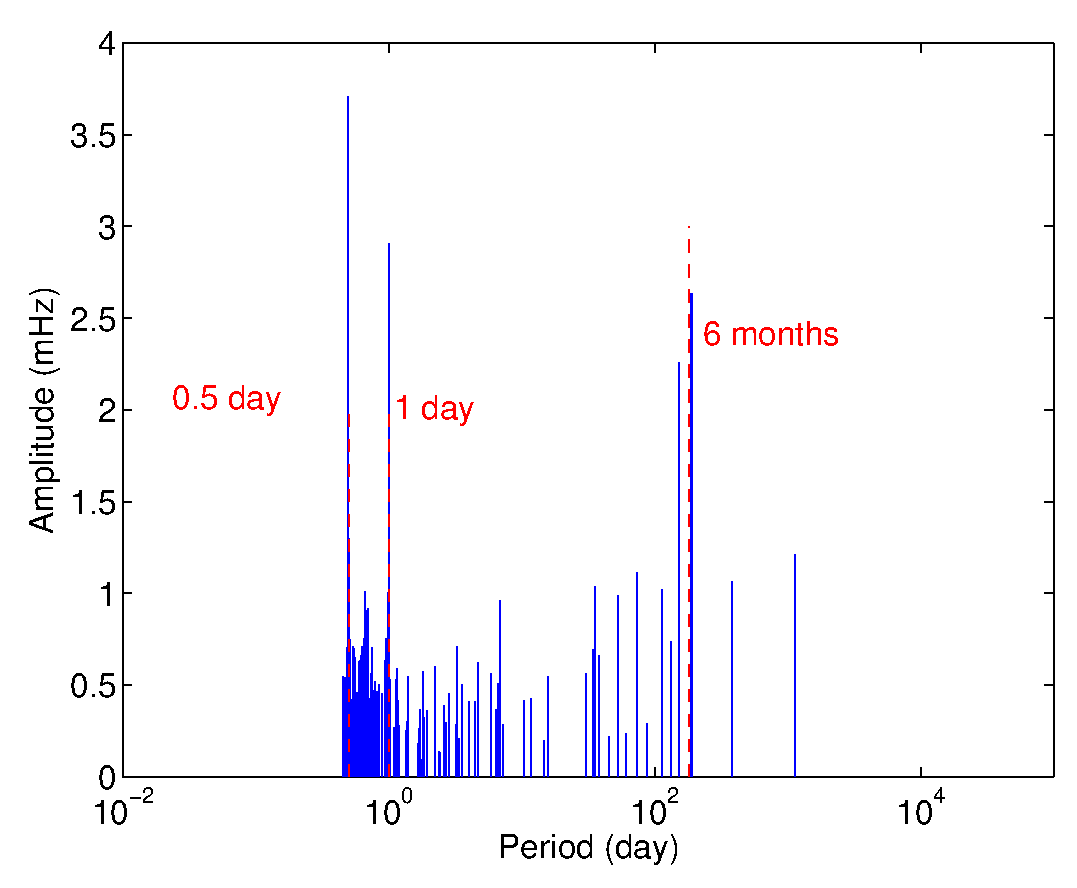
\includegraphics[width=\linewidth]{images/SparSpec_begining}
	\label{fig:SparSpec_pre}
  \caption{SparSpec Analyse der Abweichungen nach einem Fit mit konstanter Anomalie, ohne variable Terme.}
\end{minipage}
\hfill
\begin{minipage}[t]{.48\linewidth}
	\centering
	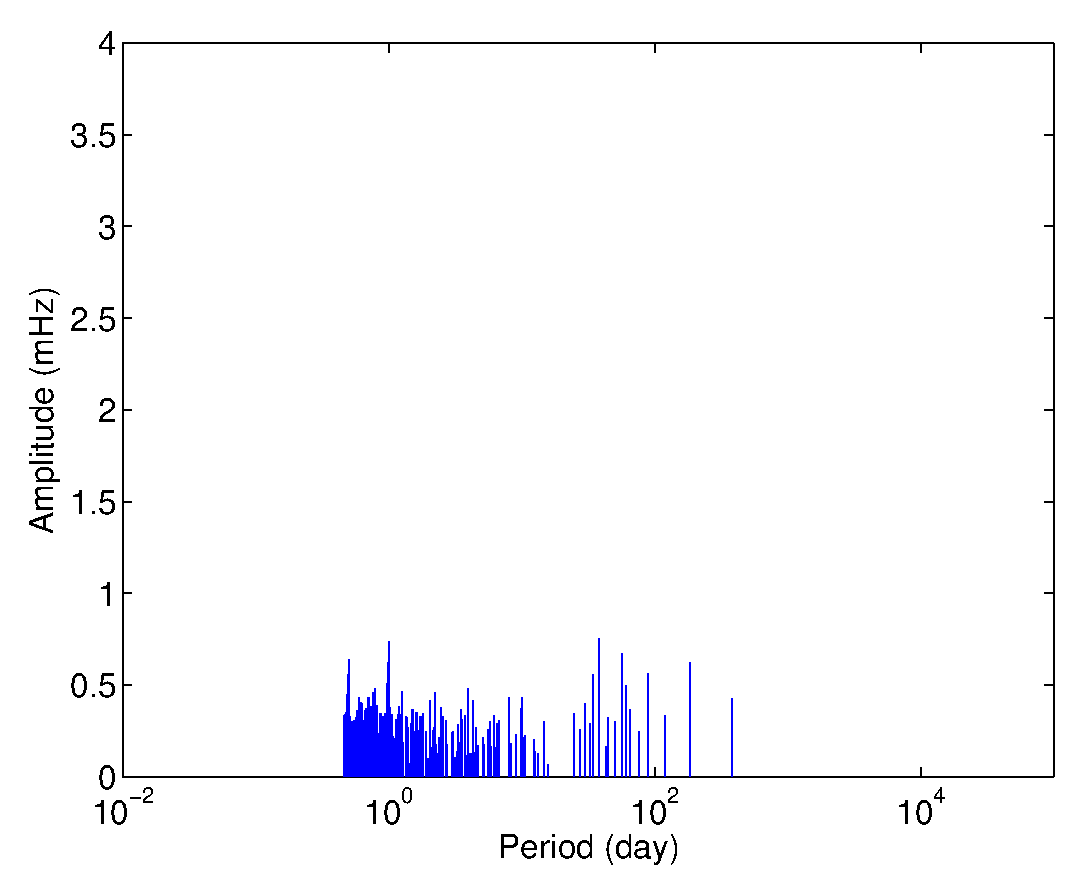
\includegraphics[width=\linewidth]{images/SparSpec_end}
	\label{fig:SparSpec_post}
  \caption{... und mit variablen Termen.}
\end{minipage}
 \end{figure}

Um die Existenz von periodischen Signalanteilen zu verdeutlichen, tragen die Abweichungen der Messwerte nach Entfernen der konstanten Anomalie im Frequenzbereich auf. Gewöhnlicherweise verwendet man dafür eine Fouriertransformation, da die Messpunkte im Falle der Pioneer-Daten allerdings nicht gleichmäßig verteilt sind, ist dies hier nicht möglich. Statt dessen verwendet man eine Software namens SparSpec.
Die periodischen Anteile des Signals lassen sich auf der daraus erhaltenen Abbildung \ref{fig:SparSpec_pre} sehr gut als herausragende Spitzen erkennen.
Die drei großen Peaks liegen bei $f_1=0.9974\pm0.004\ Tagen$, $f_2=\frac12(0.9972\pm0.004)\ Tagen$ und 
$f_3=189\pm32\ Tagen$, wobei $ 1\ Tag = 60 \cdot 60 \cdot 24 \:s = 86400\:s$ ist.
Bedenkt man das 1.0 siderischer Tag = 0.9972 Tage ist, so entspricht dies genau halbtägigen, täglichen und halbjährlichen Schwankungen.

Die Ursache für diese periodischen Terme dürfte nach gängiger Ansicht nicht in den Sonden zu suchen sein. Fehler im atmosphärischen Modell wären eine naheliegende Ursache für tägliche Variationen. Da diese jedoch von den Konditionen bei den Einrichtungen des DSN abhängen, müssten sie mit der Periode des Sonnentags und nicht des siderischen Tages verlaufen\cite{Levy2009}.
Anderson et al. ziehen für die Variationen Modellierungsfehler – wie Fehler in den Ephemeriden oder der Ausrichtung der Drehachse der Erde, oder fehlerhafte oder zu ungenaue Koordinaten der Messstationen – in Betracht\cite{Levy2009}\cite{Dittus2006}. % originalquelle?
Die Gruppe um Levey (GAP) hält dies jedoch für unwahrscheinlich, da diese Daten durch andere Beobachtungsmethoden
stark gestützt werden und es somit schwer wäre sie stark genug zu verändern um die gemessenen Effekte zu erklären. %Markward: Position offen geht auch

Sie nehmen in ihrer Untersuchung an, dass durch eine beliebige Ursache die Ausbreitung des Tracking-Signals auf
dem Weg zwischen Raumsonde und Erde verändert wird. Sie beschreiben die Ursache als Funktion des Winkels $\varphi$. Dieser wird definiert als die Differenz zwischen dem Azimutalwinkel der Antenne des DSN $\varphi_A$ und dem Azimutalwinkel der Pioneer-Sonde $\varphi_P$: $\varphi=\varphi_A-\varphi_P$. % siehe Grafik
Dieses Modell berücksichtigt also sowohl die Bewegung der Erde um die Sonne, als auch die Rotation der Erde um ihre Achse.
Die Beeinflussung des Signals wird nun mit Fourierkoeffizienten ($\upsilon_n$ und $\upsilon'_n$), beschrieben:
\begin{equation}
\Delta f = \sum_n (\upsilon_n(cos(n\varphi_u)+cos(n\varphi_d))+\upsilon'_n(sin(n\varphi_u)+sin(n\varphi_d))
\end{equation}
wobei $\varphi_u$ und $\varphi_d$ die Winkel $\varphi$ bei Up- beziehungsweise Down-link sind.
Nun können wir die die Fourierkoeffizienten sowie die konstante Anomalie an die Messwerte fitten. Wir verwenden dabei n = 1 und 2, das Hinzufügen von höheren Ordnungen bringt keine nennenswerte Verbesserung.

Dieses geometrische Modell beschreibt sowohl die täglichen als auch die jährlichen
Schwankungen und verringert die Standardabweichung der Messwerten von 9.8 mHz auf 5.5 mHz.
Auch die Spektralanalyse (Abb. \ref{fig:SparSpec_post}) dieses Fits zeigt die Verbesserung deutlich\cite{Levy2008}. % Besser zitieren
%mehr, weiter, ...

% Wie hängt das folgende mit dem obigen zusammen:
Nieto und Anderson weisen in \cite{Nieto2005} des weiteren darauf hin, das sich die jährliche zeitliche Änderung der Anomalie %von wann
grob durch eine Sinuswelle beschreiben lässt. Im Falle von Pioneer 10 hat diese eine Amplitude von $(0.525\pm0.155)\cdot10^{-8}cm/s^{-2}$ und im Fall von Pioneer 11 $(0.498\pm0.176)\cdot10^{-8}cms^{-2}$. Der Phasenunterschied der beiden Wellen beträgt 173.2°, was in etwa dem Winkelunterschied zwischen den ekliptikalen Längen\footnote{Ekliptikale Länge/Breite sind die zwei Himmelskoordinaten des ekliptikalen Koordinatensystems, welche die Ekliptik als Referenz zur Angabe der Position eines Objekts am Himmel verwendet.} der Flugrichtungen der Raumsonden entspricht, während die Amplituden etwa proportional zum Cosinus der ekliptikalen Breiten sind.

%Wohin damit:
Für die Betrachtung der veränderlichen Anteile der Anomalie muss die Kompressionszeit der Daten natürlich immer entsprechend kurz sein\cite{Nieto2005}.

\bigskip
\bigskip

\section{Zukünftige Forschung}
\subsection{Neue Analyse aller Vorhandener Daten}
Die Pioneer Sonden waren über drei Jahrzehnte im Weltall. Die Analyse von Anderson et al., 2002 betrachtete nur die Daten aus etwa 11,5 Jahren von Pioneer 10 und 3,5 Jahren von Pioneer 11. (Genaue Daten in der Tabelle \ref{tab:andersondaten})
%Die Analyse von Anderson et al., 2002 betrachtete nur die Pioneer 10-Daten in der Zeit vom 3. Januar 1987 bis zum 22. July 1998 (40 AU bis 70,5 AU) und die Pioneer 11-Daten vom 5. Januar 1987 bis zum 1. Oktober 1990 (22,4 AU bis 31,7 AU).
Jedoch empfing man bis zum 27. April 2002 brauchbare Daten von Pioneer 10. (Die Daten von Pioneer 11 waren ab Oktober 1990 nicht mehr brauchbar) Auch die anderen erwähnten Analysen bezogen sich immer auf etwa den selben Zeitraum, teils sogar weniger.

\begin{table}[h]
\centering
\begin{tabular}{|c|c|c|}
\hline & Pioneer 10 & Pioneer 11 \\ 
\hline Zeitpunkt & 3.01.1987 - 22.07.1998  & 5.01.1987 - 1.10.1990 \\ 
\hline Entfernung & 40 - 70,5 AU & 22,4 - 31,7 AU \\ 
\hline 
\end{tabular}
\caption{Die von Anderson et al. verwendeten Daten}
\label{tab:andersondaten}
\end{table}

 
\begin{sidewaystable}[hn]
\newcommand{\mc}[3]{\multicolumn{#1}{#2}{#3}}
\begin{tabular}{|c|c|c|c|c|c|c|}
\hline  & \mc{3}{c|}{Pioneer 10} & \mc{3}{c|}{Pioneer 11} \\
\hline  & Zeitraum & Entfernung & Datenpunkte & Zeitraum & Entfernung & Datenpunkte \\
\hline Anderson et al, 1998 & 1987-1995 &  &  &  &  &  \\
\hline Anderson et al, 2002 & 3.01.1987 - 22.07.1998 & 40 - 70,5 AU & 19.403 & 5.01.1987 - 1.10.1990 & 40 - 70,5 AU & 10.252 \\
\hline … &   &   &   &   &   &   \\
\hline Verfügbar & -27.4.2002 &  &  & -10.1990 &  &  \\
\hline 
\end{tabular}
\caption{Übersicht über die Verwendeten Daten in allen Analysen}
\label{tab:andersondaten}
\end{sidewaystable}


Die Daten von Pioneer 10 aus dem Zeitraum von 1998 bis 2002 wurden also noch nicht untersucht. Noch
Erfolgversprechender wäre jedoch eine Analyse der frühen Daten. Die Anomalie wurde bereits ab 1979 beobachtet und durch
bessere Berechnung des solaren Strahlungsdruck könnten auch die noch früheren Daten wichtige Informationen liefern.

Es ist daher bereits seit längerem geplant die kompletten Daten, vom Start der Sonden, bis zu den letzten verwertbaren Signalen neu zu analysieren. Dies stellte sich jedoch als schwerer heraus als gedacht. Als Grund dafür werden veraltete Dateiformate, fehlende Daten und beschädigte Dateien genannt.\cite{Turyshev2010}

% Es ist geplant am ZARM in Zusammenarbeit mit dem JPL die gesammten Pioneer Daten vom Start bis zum letzten Signal neu
% zu analysieren	% aus Physikjournal
% die alten Daten wurden von Magnetbändern heruntergeladen und für neue Datenanalysen vorbereitet % aus Physikjournal


\bigskip
…
\bigskip


\subsection{Die Bedeutung der Richtung der Anomalen Beschleunigung}
\bigskip
…
\bigskip


\bigskip


% ToDo:
%% - S-Band ist für 3-D wenig geeignet. (Route to Understanding)  -> ?
%% - ''Model of observation stations`` -> Messung
%% - Abgrenzung Navigation <> Einleitung
%% - ...

% ToFix:
%% - Quellen: And -> und
%% - Quellen: Großschreibung nicht ruinieren.
%% - Footnote der Authoren

\bibliography{lit}{}
\bibliographystyle{unsrtdin}

\end{document}
